\clearpage
\bigsection{Evaluation}
% TODO How much time spend benchmarking
Games: Ashes of the Singularity which will sometimes be abbreviated as \emph{Ashes} in the following, Dota 2, F1 2017, Mad Max and Warhammer 40,000: Dawn of War III which we will shorten to Warhammer.

\subsection{Basic Block Counters}
\label{sub:eval_counters}
Shaders are small programs compared to CPU programs, more like a single function. This means the number of basic blocks in a shader is low as seen in \cref{dia:shader_bbs_dota}.
LLVM uses the counters e.g. for linearization. A performance comparison using the default optimizations in LLVM that rely on PGO data is shown in \dots. The optimizations do not change the performance of the selected games significantly.

The basic block counters influence order of basic blocks -> No impact on performance on most shaders?
Marks pixel shaders as hot and vertex shaders as unlikely.

To get an intuition for the counter values we get, \cref{dia:counter_values} displays a histogram.
The x-axis of this diagram represents the counter, i.e. how often a basic block is executed.
A bar for the execution counts 20--30 for example represents all blocks which get run at least 20 times but at max 30 times (excluded).
The high of the bar counts how many basic blocks fall into this range.
Lots of blocks fall into the lowest bucket of the diagram, the leftmost bar. This bar is cut off, otherwise the rest of the bars would not be visible.
This means most basic blocks get executed less than $10^6$ times. A few blocks run a lot more often, more than $10^12$ times.

\begin{figure}
\pgfplotsset{width=\textwidth}
\centering
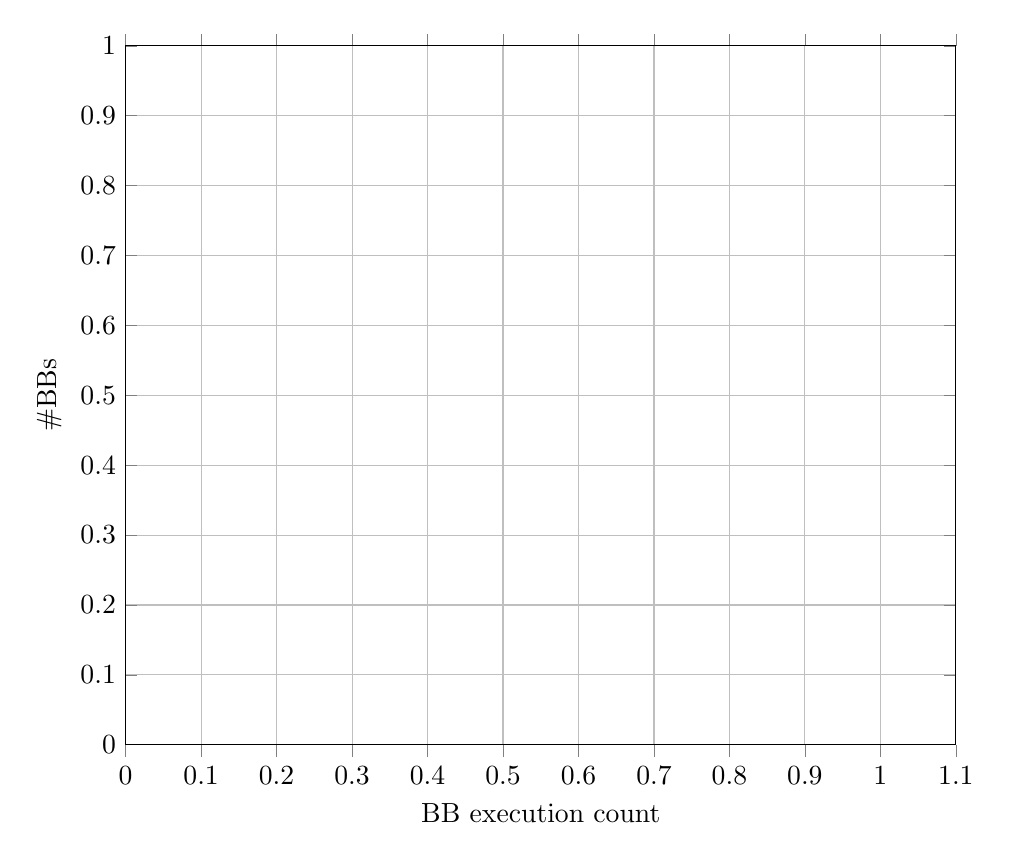
\begin{tikzpicture}
\begin{axis}[
	ybar,
	xlabel={BB execution count},
	ylabel={\#BBs},
	xmin=0,
	ymin=0,
	ymax=20,
	grid=both,
	%bar width=0.5cm,
]

\runtex{counter-dist1 -g dota}

\node at (axis cs:15e9,19) {\color{white}↑};
\end{axis}
\end{tikzpicture}
\captionof{figure}{The distribution of counter values on basic blocks of Dota 2}
\label{dia:counter_values}
\end{figure}

\begin{figure}
\pgfplotsset{width=\textwidth}
\centering
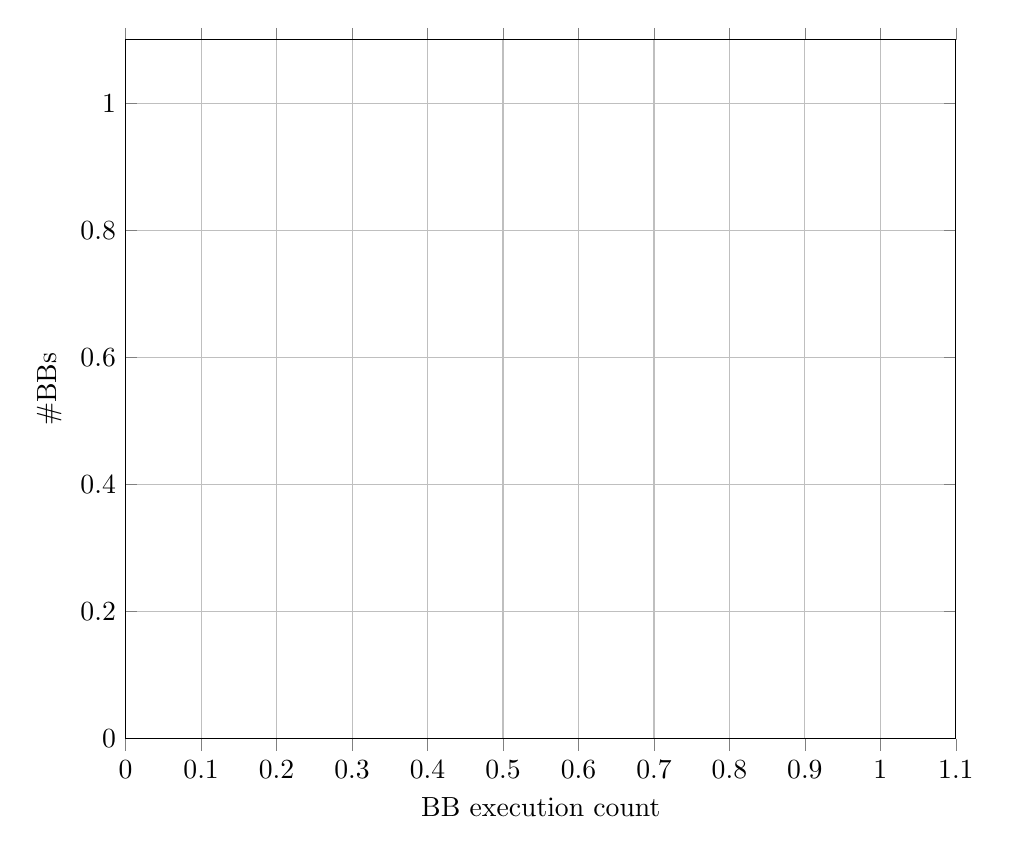
\begin{tikzpicture}
\begin{axis}[
	ybar,
	xlabel={BB execution count},
	ylabel={\#BBs},
	xmin=0,
	ymin=0,
	grid=both,
	%bar width=0.5cm,
]

\runtex{counter-dist2 -g dota}
\end{axis}
\end{tikzpicture}
\captionof{figure}{The distribution of counter values on basic blocks of Dota 2}
\label{dia:counter_values}
\end{figure}


\subsection{Unused code}
\label{sub:eval_unused}
We test the effect of removing unused code with a small sample program which runs a bytecode virtual machine in a shader with one large switch-case statement.
The bytecode computes the final fragment color and in our example only uses a single bytecode instruction out of 71 possible instructions.
Using PGO, we detect that all other instructions are never executed and in the optimized shader version we remove all these basic blocks.
This leaves us with compare and jump instructions from the original binary jump tree but only one of the branch instructions is taken and the code has a lot less basic blocks than before.

\newcommand\unuseddiag[2]{
\begin{figure}
\pgfplotsset{width=\textwidth,height=7cm}
\centering
\begin{tikzpicture}
\begin{axis}[
	ybar,
	xlabel={\#BBs in a Shader},
	ylabel={Unused BBs [\SI{}{\percent}]},
	xmin=0,
	xmax=\runtex{max-bbs -g #1},
	ymin=0,
	ymax=100,
	ytick pos=left,
	grid=both,
	bar width=0.01cm,
]

\runtex{unused-code -g #1}
\end{axis}

\begin{axis}[
	axis y line*=right,
	axis x line=none,
	xlabel={\#BBs in a Shader},
	ylabel={Distribution of shaders [\SI{}{\percent}]},
	xmin=0,
	xmax=\runtex{max-bbs -g #1},
	ymin=0,
	legend style={at={(1,1)},anchor=north east},
]
\addlegendimage{only marks, fill=gray, draw=gray, fill opacity=0.4}\addlegendentry{Shader distribution}
\runtex{bbs -g #1}
\addlegendentry{Shader with unused BBs}
\end{axis}
\end{tikzpicture}
\captionof{figure}{The fraction of unused code by shader size in #2}
\label{dia:unused_by_bb_#1}
\end{figure}
}

\unuseddiag{ashes}{Ashes}
\unuseddiag{dota}{Dota 2}
\unuseddiag{f12017}{F1 2017}
\unuseddiag{madmax}{Mad Max}
\unuseddiag{dow3}{Warhammer}
\unuseddiag{switch}{the switch vm}

\begin{figure}
\pgfplotsset{width=\textwidth}
\centering
\begin{tikzpicture}
\runtex{unused-code-summary}
\end{tikzpicture}
\captionof{figure}{The fraction of unused basic blocks per game}
\label{dia:unused_by_game}
\end{figure}


Register usage, split by shader type.
For each game in three configurations: Running the game without any special options, using profile-guided optimizations and using PGO with removing unused basic blocks.
\begin{figure}
\pgfplotsset{width=\textwidth}
\centering
\begin{tikzpicture}
\begin{axis}[
	ybar,
	xlabel={Game},
	ylabel={\#Registers used},
	xmin=0,
	xmax=40,
	grid=both,
	axis lines=left,
	bar width=0.5cm,
]

\addplot [
	fill=tumblue,
] table {data/dota_bbs.txt};
\end{axis}
\end{tikzpicture}
\captionof{figure}{Register usage in compute shaders}
\label{dia:registers_cs}
\end{figure}

\begin{figure}
\pgfplotsset{width=\textwidth}
\centering
\begin{tikzpicture}
\begin{axis}[
	ybar,
	enlarge x limits=0.4,
	symbolic x coords={dota,ashes},
	xticklabels={Dota 2,Ashes of the Singularity},
	xtick=data,
	ylabel={\#Registers used},
	ymin=0,
	grid=both,
	nodes near coords,
	every node near coord/.append style={rotate=90, anchor=west},
	bar width=0.5cm,
	legend style={at={(1,1)},anchor=north east},
]

\addplot [
	fill=tumblue,
] table[header=false] {data/registers-cs.txt};
\end{axis}
\end{tikzpicture}
\captionof{figure}{Register usage in vertex shaders}
\label{dia:registers_vs}
\end{figure}

\begin{figure}
\pgfplotsset{width=\textwidth}
\centering
\begin{tikzpicture}
\begin{axis}[
	ybar,
	xlabel={Game},
	ylabel={\#Registers used},
	xmin=0,
	xmax=40,
	grid=both,
	axis lines=left,
	bar width=0.5cm,
]

\addplot [
	fill=tumblue,
] table {data/dota_bbs.txt};
\end{axis}
\end{tikzpicture}
\captionof{figure}{Register usage in fragment shaders}
\label{dia:registers_fs}
\end{figure}


% TODO Scatter plot

\subsection{Uniform Branches}
\label{sub:eval_uniform_branches}

\begin{figure}
\pgfplotsset{width=\textwidth}
\centering
\begin{tikzpicture}
\begin{axis}[
	ybar stacked,
	enlarge x limits=0.2,
	cycle list name=mycolors,
	symbolic x coords={ashes,dota,dow3,f12017,madmax},
	xticklabels={Ashes,Dota 2,Warhammer,F1 2017,Mad Max},
	xtick=data,
	ylabel={Uniformity [\SI{}{\percent}]},
	ymin=0,
	ymax=100,
	grid=both,
	nodes near coords,
	% Do not display text for nodes with value < … by setting opacity to 0
	node near coords style={
		/utils/exec={\setbox0\hbox{\pgfmathprintnumber\pgfplotspointmeta}
		\pgfmathfloattomacro{\pgfplotspointmeta}{\F}{\M}{\E}
		\pgfmathsetmacro{\myopacity}{ifthenelse(\M*pow(10,\E)<17,0,1)}
		},
		rotate=90, anchor=center, opacity=\myopacity},
	bar width=0.5cm,
	legend style={at={(1,1)},anchor=south east},
]

\runtex{uniform-branches}
\legend{Static uniform,Dynamic uniform,Divergent}
\end{axis}
\end{tikzpicture}
\captionof{figure}{Uniformity of branches}
\label{dia:uniform_branches}
\end{figure}


\subsection{Uniform Loads}
\label{sub:eval_uniform_loads}

\centering
\begin{tikzpicture}
\begin{axis}[
	ybar stacked,
	enlarge x limits=0.2,
	cycle list name=mycolors,
	symbolic x coords={ashes,dota,dow3,f12017,madmax},
	xticklabels={Ashes,Dota 2,Warhammer,F1 2017,Mad Max},
	xtick=data,
	ylabel={Uniformity [\SI{}{\percent}]},
	ymin=0,
	ymax=100,
	grid=both,
	nodes near coords,
	% Do not display text for nodes with value < … by setting opacity to 0
	node near coords style={
		/utils/exec={\setbox0\hbox{\pgfmathprintnumber\pgfplotspointmeta}
		\pgfmathfloattomacro{\pgfplotspointmeta}{\F}{\M}{\E}
		\pgfmathsetmacro{\myopacity}{ifthenelse(\M*pow(10,\E)<17,0,1)}
		},
		rotate=90, anchor=center, opacity=\myopacity},
	bar width=0.5cm,
	legend style={at={(1,1)},anchor=south east},
]

\runtex{uniform-loads}
\legend{Static uniform,Dynamic uniform,Divergent}
\end{axis}
\end{tikzpicture}


\subsection{Performance}
\label{sub:eval_perf}
Performance comparison in three configurations: Running the game without any special options, using profile-guided optimizations and using PGO with removing unused basic blocks.

\begin{tikzpicture}
\begin{axis}[
	ybar,
	enlarge x limits=0.1,
	cycle list name=mycolors,
	symbolic x coords={ashes,dota,dow3,f12017,madmax,switch},
	xticklabels={Ashes,Dota 2,Warhammer,F1 2017,Mad Max,Switch vm},
	xtick=data,
	xticklabel style={text width=2cm,align=center},
	ylabel={{\color{tumblue}$\blacktriangleleft$} less is better, Time per frame [\SI{}{\milli\second}]},
	ylabel style={align=center},
	ymin=0,
	grid=both,
	%nodes near coords,
	%every node near coord/.append style={rotate=90, anchor=west},
	bar width=0.3cm,
	legend style={at={(1,1)},anchor=north east, font=\scriptsize},
	point meta=explicit symbolic,
	nodes near coords={\pgfplotspointmeta},
	every node near coord/.append style={yshift=0.2cm, font=\scriptsize},
]

\runtex{performance-presentation}
\end{axis}
\end{tikzpicture}


\subsection{Overhead}
\label{sub:overhead}
To find hot paths, the instrumentation inserts counters into some basic blocks of a program. The counters introduce an overhead, compared to a non-instrumented version of the code.
In the case of counting the frequency of basic block executions, the counters themselves are not sensitive to timing and thus not directly influenced by this overhead.
But the code will run slower. In the case of a game, we will observe fewer frames per second than usual.
If the benchmark, that we run with PGO instrumentation, runs for a fixed time, we will get lower basic block frequencies for fewer frames per second.
Therefore, the measured counters may be less than the actual frequencies that we try to measure.

We measured the overhead for two different games in different configurations: Dota 2 and Ashes of the Singularity. The baseline in \cref{dia:overhead} and \cref{tab:overhead} is a normal run of the game with no counters.
The first tested configuration uses normal add instructions (i.e. no atomics) and increments by one per SIMD unit.
The second and third variant use atomic counters, either incrementing by one on each SIMD lane or once per unit.
All instrumentation was inserted after structurizing the CFG.

As expected, incrementing per lane needs the most time. An atomic add causes less overhead for Dota 2 than the non-atomic version.
The reason is that the non-atomic increment needs a load and a store operation where the atomic version needs only a single memory transaction. The actual addition is computed inside the L2 cache for atomics.
For Ashes of the Singularity, we cannot see much of a difference in performance. The per-lane variant is significantly slower but only by \SI{0.25 \pm 0.06}{\percent}.

\begin{figure}
\centering
\pgfplotsset{width=\textwidth}
\centering
\begin{tikzpicture}
\begin{axis}[
	ybar,
	enlarge x limits=0.2,
	cycle list name=mycolors,
	symbolic x coords={ashes,dota,dow3,f12017,madmax},
	xticklabels={Ashes,Dota 2,Warhammer,F1 2017,Mad Max},
	xtick=data,
	ylabel={\footnotesize {\color{tumblue}$\blacktriangleleft$} Time per frame [\SI{}{\milli\second}], less is better},
	ymin=0,
	grid=both,
	%nodes near coords,
	%every node near coord/.append style={rotate=90, anchor=west},
	bar width=0.5cm,
	legend style={at={(1,1)},anchor=north east},
]

\runtex{overhead -d}
\end{axis}
\end{tikzpicture}
\captionof{figure}{Overhead of BB counters}
\label{dia:overhead}
\end{figure}


% TODO Why ashes? Code size / BB-count

\begin{table}
\centering
\runtex{overhead}
\captionof{table}{Overhead of BB counters}
\label{tab:overhead}
\end{table}


In some cases, it may be necessary to decrease the overhead of basic block counters. For example to use the instrumentation in production environments where high overheads are not acceptable.
Sometimes, the overhead is high enough to trigger timeouts in the GPU driver, leading to game crashes. This is the case for the Infiltrator demo project of the Unreal Engine.

A simple way to decrease the overhead is to switch from atomic counters to non-atomic counting. This is enough to let e.g. the Infiltrator demo start, however it comes with a drawback. Shaders are executed highly parallel, so many instances of a shader will simultaneously access the same memory location of a counter.
These race conditions lead to inaccurate counters. Not only do we get wrong proportions of frequencies, we also have to take into account that not every basic block gets a counter, some frequencies are computed from multiple counters. This leads to cases where basic blocks that are not executed at all at runtime are assigned a counter value of several thousand executions because the counter values used to compute the frequencies are inaccurate.

Another overhead reduction can be achieved by skipping counting on most SIMD units and activate it e.g. only on \SI{5}{\percent} of the units.
This means most executions will skip the increments, having even less overhead than the non-atomic variant while the rest of the executions gives accurate statistics.
A problem with this approach is that (e.g. vertex-) shaders that get executed only a few times, might not land on any of SIMD units where counting is activated and we get no statistics at all for them.
This should only be a small problem because these shaders probably do not account for much of the computation time (as they are executed only a few times) and optimizing them cannot yield big benefits anyway.

A more sophisticated technique that can speed up basic block counting tries to reduce the memory pressure by atomics without falling back to non-atomic counting. As we know, many atomic operations will simultaneously try to access the same memory location.
We can reduce this pressure if we add multiple memory locations in different cache lanes for the same counter and spread the counting over these locations. As less atomic increments access the same memory, they do not have to wait as long as before and the program execution can continue faster.
In the end, when shutting down the application, we have to add up all duplicated counters. This happens only once in the end for most applications so it adds not much overhead.
